\chapter{Post-Processing Techniques for Instance Segmentation Masks}\label{ch:postProcessing}

At this stage, the system is capable of detecting cetaceans at an individual pixel level. Before these detections can be passed to the identification module, some post-processing of the output must be performed to allow for both a reduction in the computational expense of operating on the detector's output as well as ensuring that no potentially important information which will assist in an identification is lost. 

\section{Handling Multiple Detections}\label{ch:postProcessing,sec:handlingMultipleDetections}

When an image is ran through the Mask-RCNN detector \cite{he_mask_2017}, the number of outputs can vary depending on how many detected objects have a confidence score higher than 90\% (as discussed in Section \ref{ch:cetDet,sec:ModelSelection,sub:DetectionHyperparameters}). If no detections reach this threshold the image is discarded from further processing. This can occur if, for example, an image is taken by accident capturing the vessel's floor. If a single detection reaches the threshold, the resultant mask is passed downstream. 

Thanks to the tendency for cetaceans to travel in pods however, it is unlikely an image will contain only a single \texttt{dolphin} detection. In these situations the Mask-RCNN will output multiple detections masks, one per object. To handle this, the first stage of the post-processing methodology is to separate multiple detections for a single image. This ensures each \texttt{dolphin} detection is handled independently, mitigating the potential for an identification to be influenced by the others. An example of this behaviour can be seen in Figure \ref{fig:190730-001-MOLS0360_-detections}. Here, an image inputted to the Mask-RCNN detector has produced three detections which are above the threshold. As such, they have been split into three output masks for individual processing. Note that one of the masks, indicated in blue in the Top Left figure, has been incorrectly detected as \texttt{dolphin} with a high confidence. As such a mask has been produced, visualised Bottom Right. The downstream components of the system must thus be capable of handling background which has been incorrectly labelled, ideally via further post processing before the identification stage. 

\begin{figure}[h]
	\begin{center}
		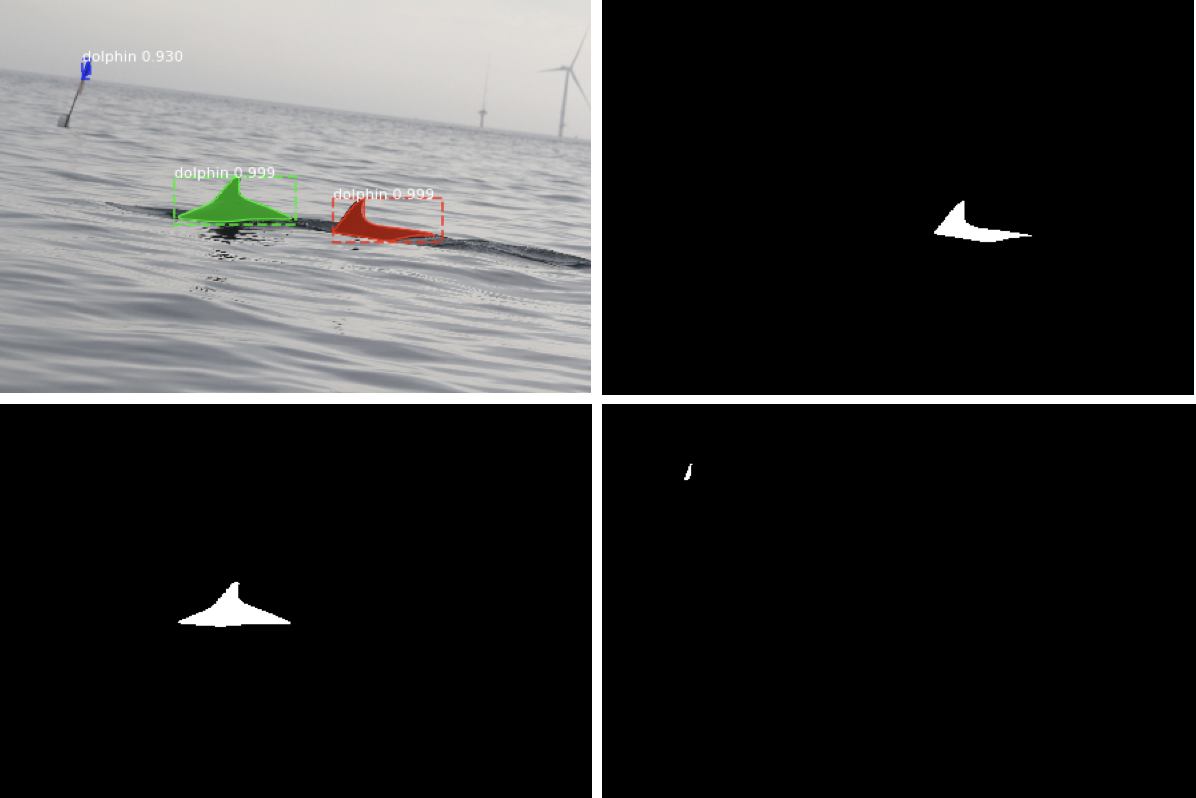
\includegraphics[scale=0.5]{Chapter4/figs/190730-001-MOLS0360_-detections.png}
	\end{center}
	\caption{Top Left: A visualisation of the three \texttt{dolphin} detections for an input image produced by the Mask-RCNN detector, alongside their confidence scores. Top Right, Bottom: The resultant detection masks once split, where \texttt{dolphin} is displayed in white.}
	\label{fig:190730-001-MOLS0360_-detections}
\end{figure}


\section{Morphological Transformations}\label{ch:postProcessing,sec:morphologicalTransformations}

In some situations a detected mask may contain an area of background inside the detection. This can be thought of as a hole in the detection, as seen in Figure \ref{fig:before-and-after-morphing-masks-only} (Left). Using \textit{a priori} knowledge of cetaceans, it can be deduced that a hole in the detection is highly unlikely and causes a loss of potentially useful identifying information. As such, any holes which are present in the masks must be removed. 

\begin{figure}[h]
	\begin{center}
		
\includegraphics[scale=0.5]{Chapter4/figs/before-and-after-morphing-masks-only.png}
	\end{center}
	\caption{Left: A detection mask before morphological transformations have been applied. The detected \texttt{dolphin} object is displayed in white. Note the cluster of black background pixels inside. Right: The same detection mask after morphological transformations have been applied. Note the pixels which make up the hole have been converted to \texttt{dolphin}.}
	\label{fig:before-and-after-morphing-masks-only}
\end{figure}

This is achieved using morphological transformations, a set of operations which allow for the automated manipulation of the internal structure of a binary image such as masks. The two fundamental morphological transformations are called erosion, which erodes away the boundaries of the masked object, and dilation, which increases the size of the object by pushing the boundary out into the background space. These two operations can be utilised in various combinations to perform other useful transformations.

In order to remove the cluster of background pixels inside of the detection, each mask is \textit{closed} - dilated then eroded. This has the effect of removing any holes present inside the mask. If no holes exist, the operation is still performed however the mask remains unchanged. By performing closing, the system ensures that no potentially identifiable information is lost as a result of an incomplete detection. This effect can be seen in Figure \ref{fig:before-and-after-morphing-masks-only} (Right).

\section{Background Subtraction}\label{ch:postProcessing,sec:bgExtraction}

Now that the mask has been cleaned using morphological transformations, it is possible to utilise it to perform background subtraction. This is an extremely important step in ensuring an accurate individual classification based on the detected \texttt{dolphin} object, ensuring no background noise is passed to the identification system which may influence the final classification.

As both the input image and resultant mask can be represented as matrices, these can be manipulated utilising a \textit{bitwise and} operation such that if pixel$_{i, j}$ in the input image is denoted as background in the mask, the values of pixel$_{i, j}$ can be set to [255, 255, 255] (white). This has the effect of whiting out any pixels not detected as part of the \texttt{dolphin} in the input, whilst keeping the pixels detected as \texttt{dolphin} intact.

An example of background subtraction utilising cleaned masks can be seen in Figure \ref{fig:190730-001-MOLS0360_-bg-subtraction}. Using the same input image as in Figure \ref{fig:190730-001-MOLS0360_-detections}, it can be seen that the \textit{bitwise and} operation whites all pixels in the image except those which have been classified as \texttt{dolphin} for each of the three output masks. Note at this point however that the erroneous classification, shown Bottom Right, still remains. 

\begin{figure}[h]
	\begin{center}
		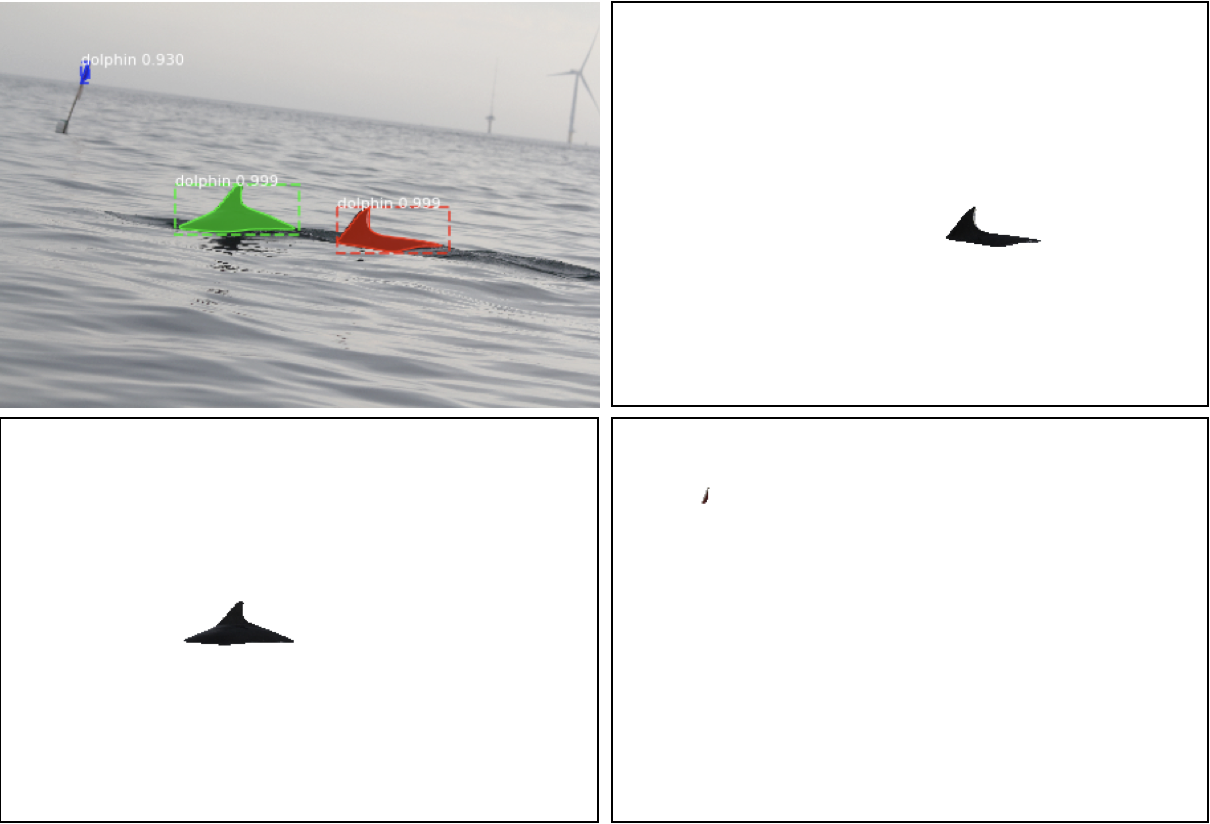
\includegraphics[scale=0.5]{Chapter4/figs/190730-001-MOLS0360_-bg-subtraction.png}
	\end{center}
	\caption{Top Left: A visualisation of the three \texttt{dolphin} detections for an input image produced by the Mask-RCNN detector, alongside their confidence scores. Top Right, Bottom: The resultant output images after \textit{bitwise and} operations performed between the input image and the cleaned detection masks. A border has been added for clarity.}
	\label{fig:190730-001-MOLS0360_-bg-subtraction}
\end{figure}

% Show that it may not be possible to remove all background pixels if the mask includes them, images below but uncropped. 

Whilst the background subtraction aims to reduce noise passed downstream to the individual identification module, it will not be possible to remove all noise. It may be the case, such as in Figure \ref{fig:fin-extraction-unclean}, whereby some background has been mislabelled as \texttt{dolphin}. As a result, the background subtraction module is unable to remove the mislabelled background pixels which may effect the accuracy of the identification downstream unless the system is robust enough to deal with this.

%% TODO: fin-extraction-unclean input img, or other good example of fin with some bg present.
\begin{figure}[h]
	\begin{center}
		\includegraphics[scale=0.5]{example-image}
	\end{center}
	\caption{The result of background subtraction and cropping where the detector has mislabelled some background pixels as \texttt{dolphin}, right. Detected pixels have been highlighted red on the input image, left, with confidence score shown.}
	\label{fig:fin-extraction-unclean}
\end{figure}



\section{Colour Thresholding}\label{ch:postProcessing,sec:splittingByComponent}

As the Mask-RCNN detector is not perfect, it may sometimes incorrectly classify background as a \texttt{dolphin} object. An example of this can be seen in Figure \ref{fig:190730-001-MOLS0360_-detections}, where a flag denoting the location of a lobster pot has been incorrectly identified as a \texttt{dolphin} object with high confidence rather than as background. As a result, any post-processing methodology must be capable of not only cleaning detections to improve the chance of individual identification, but also remove erroneous detections before they reach the identifier. 

% Discuss colour thresholding. 90% global, then for each fin are 50% of the pixels above that.
% Examples from below


\section{Cropping}\label{ch:postProcessing,sec:cropping}


%=================
%
%\section{Background Subtraction \& Cropping}\label{ch:postProcessing,sec:bgExtraction}
%
%One of the main components of the post-processing pipeline is the background subtraction module. 
%
%As both the input image and its resultant mask can be represented as matrices, these can be manipulated utilising a \textit{bitwise and} operation such that if pixel$_{i, j}$ in the input image is denoted as background in the mask, the values of pixel$_{i, j}$ can be set to [255, 255, 255] (white). This has the effect of whiting out any pixels not detected as part of the fin in the image, removing noise. 
%
%Once the background subtraction has been achieved the input image can then be cropped to reduce file size. By using the top, bottom, left, and right-most non-white pixels in the image as bounding box coordinates for the fin, the input image can be vastly reduced, often to only a few hundred pixels in both height and width. This greatly reduces the computational expense of further operations downstream by reducing the size of subsequent input images passed to other components. 
%
%Figure \ref{fig:fin-extraction-clean} shows the effect of performing background subtraction on an input image, with the detected \texttt{dolphin} pixels from the Mask-RCNN highlighted in red. As can be seen, the background subtraction and cropping has resulted in a clean image of the animal's dorsal fin. Identifying information is present, with minimal levels of noise. 
%
%\begin{figure}[h]
%	\begin{center}
%		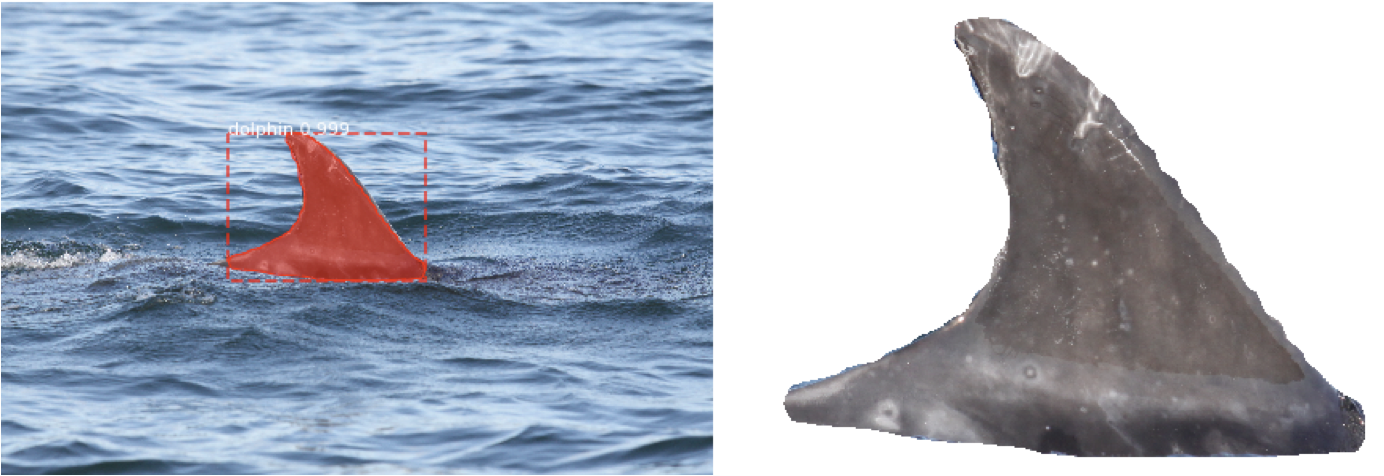
\includegraphics[scale=0.5]{Chapter4/figs/fin-extraction-clean.png}
%	\end{center}
%	\caption{The effect of background subtraction and cropping on an input image, left. The detected \texttt{dolphin} pixels by the Mask-RCNN have been highlighted in red with confidence score shown. The resultant output, right, has been enlarged for visibility.}
%	\label{fig:fin-extraction-clean}
%\end{figure}
%
%Whilst the background subtraction module aims to reduce as much noise as possible entering the identification module, which can be achieved thanks to the high accuracy of the detector, it will not be possible to remove all noise. It may be the case, such as in Figure \ref{fig:fin-extraction-unclean}, whereby some background has been mislabelled as \texttt{dolphin}. As a result, the background subtraction module is unable to remove the mislabelled background pixels which may effect the accuracy of the identification downstream unless the system is robust enough to deal with this.
%
%\begin{figure}[h]
%	\begin{center}
%		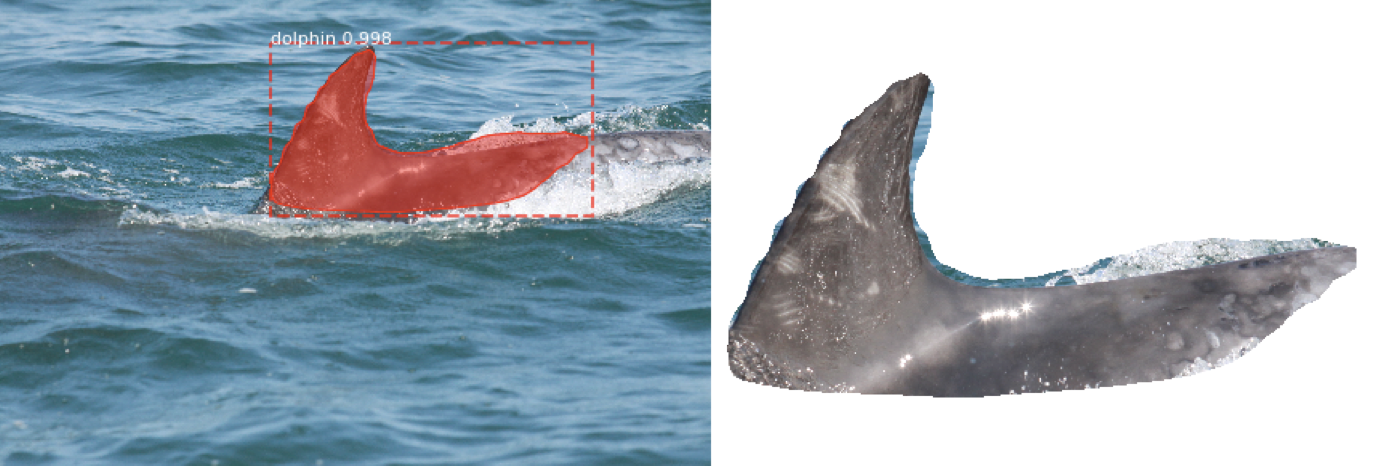
\includegraphics[scale=0.5]{Chapter4/figs/fin-extraction-unclean.png}
%	\end{center}
%	\caption{The result of background subtraction and cropping where the detector has mislabelled some background pixels as \texttt{dolphin}, right. Detected pixels have been highlighted red on the input image, left, with confidence score shown.}
%	\label{fig:fin-extraction-unclean}
%\end{figure}
%
%As cetaceans often travel in pods containing multiple individuals, any post-processing methodology must be capable of handling this. To account for this, if the background subtraction module is passed multiple masks for an image it operates on each mask independently. This results in potentially multiple output images per input, one for each detection. An example of this behaviour can be seen in Figure \ref{fig:fin-extraction-pod-with-flag}.
%
%\begin{figure}[h]
%	\begin{center}
%		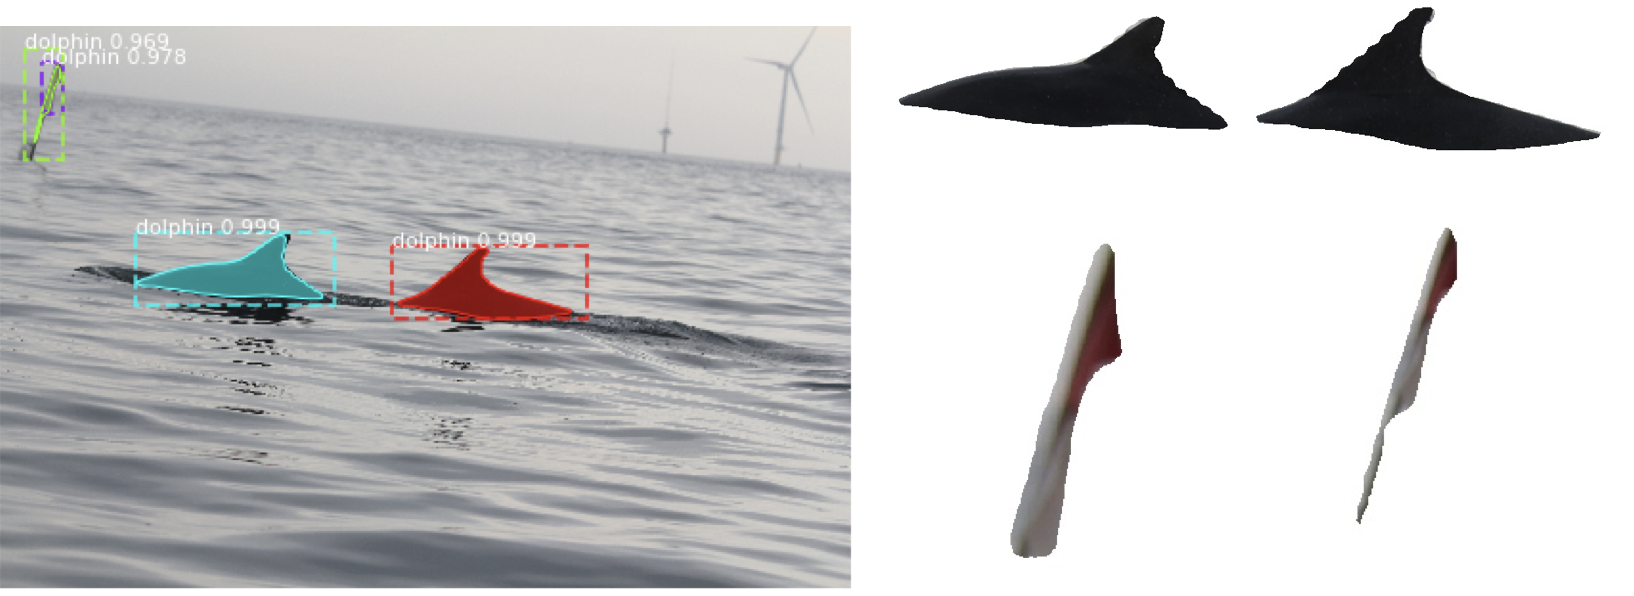
\includegraphics[scale=0.5]{Chapter4/figs/fin-extraction-pod-with-flag.png}
%	\end{center}
%	\caption{The result of background subtraction and cropping where the detector is passed multiple masks for an input image, right. Detections and confidence scores are overlaid onto the input image, left.}
%	\label{fig:fin-extraction-pod-with-flag}
%\end{figure}
%
%As the Mask-RCNN has detected four \texttt{dolphin} objects in the image, the background subtraction and cropping module has produced four output images. However it can be seen that two of the detections have been misclassified - they are actually of a flag denoting the location of a lobster pot and thus should be background. Further post-processing of the detection outputs is required to ensure the minimal amount of erroneous detections are passed downstream without stopping correct classifications. 
%
%
%
%% Rejig this chapter to follow format in Log 16/3


%%%%%%%%%%%%%%%%%%%
\nomenclature[z-CNN]{CNN}{Convolutional Neural Networks}

